\chapter{Machine learning foundations}

The aim of this chapter is to introduce the methods of machine learning, which
are going to be used for the purposes of predictive regression modeling in 
this thesis. The chapter starts with a brief overview of machine learning as
a method, followed by descriptions of the individual algorithms used.

\section{Machine learning as a method}

Nowadays, we can say that machine learning (ML) has become a buzzworthy term in
the field of data science. It stands for the subset of artificial intelligence enabled to identify patterns in data \cite{ibm}.
Generally speaking, ML implements algorithms capable of learning from data and generalizing patterns to be able to make predictions on unseen data,
which means being able to perform tasks without being explicitly told to \cite{islp}.      

Mathematically speaking, ML builds on the idea of having a quantitative target variable $Y$ and $p$ various
predictors $X_1, X_2, \ldots, X_p$. We assume the existence of an underlying function $f$ such that

\begin{equation}
Y = f(X_1, X_2, \ldots, X_p) + \epsilon,
\end{equation}

where $\epsilon$ is a random noise independent of $X_1, X_2, \ldots, X_p$. Algorithms and methods of ML 
aim to estimate the function $f$ by using a so-called \textbf{training dataset} of observed data. 

Suppose we have $n$ observations of the introduced predictors and the corresponding target $Y$ as $\{ Y_i, X_{i, 1}, X_{i, 2}, \ldots, X_{i, p} \}_{i=1}^{n}$, where $X_{i, q}$ denotes value of the $q$-th predictor in the $i$-th observation.
Then, ML algorithms use this dataset to approximate function $\hat{f}$, such that $\hat{f}(X_{i, 1}, X_{i, 2}, \ldots, X_{i, p}) = \hat{Y}_i \approx Y_i$, for all $i=1, 2, \ldots, n$. With the obtained $\hat{f}$, we can make predictions of $Y$ for new (unseen before) values of predictors $X_1, X_2, \ldots, X_p$.
\newline
\par
Based on the methodology used to find $\hat{f}$, we can distinguish two methods – \textit{parametric} and \textit{non-parametric}. 
\textbf{Parametric methods} seek to approximate $f$ by specifically optimizing a various number of parameters, which then explicitly define the function $\hat{f}$. This involves a prior assumption
about the functional form of $f$ (e.g., linear, polynomial, etc.). Then, using specific algorithms, the parameters of the function are estimated from the training data, resulting in $\hat{f}$. Examples of
such methods used in this thesis are linear regression or its regularized variants. 

On the other hand, \textbf{non-parametric methods} do not assume any specific functional form of $f$. Instead, they rely on patterns included in the data itself to roughly approximate $f$. Generalisation to unseen data
is achieved by identifying patterns and similarities in the training data, without explicitly defining $\hat{f}$. An example of such a method used in this thesis is the k-nearest neighbours algorithm or the random forest algorithm.

Next, based on the character of the $Y$, we can distinguish \textit{regression} and \textit{classification} tasks. In \textbf{regression} tasks, $Y$ is a continuous variable, while in \textbf{classification} tasks, $Y$ is a discrete variable.

Lastly, in order to have a complete picture of ML theory foundations, it is important to mention the terms \textit{overfit} and \textit{underfit} learning. In the process of building the model to approximate $f$,
we might encounter such a phenomenon, where the trained model captures patterns in the training dataset very well (memorizes), but, on the other hand, on a set of unseen data fails in terms of accuracy – this is called \textbf{overfit}. In contrast, \textbf{underfit}
comes when the model and resulting $\hat{f}$ fail to generalize patterns on both training and unseen sets.
   
\section{Linear regression}

Linear regression is undoubtedly the most fundamental method in ML. It is a parametric method used for regression tasks, assuming that the true relationship between the predictors and the target variable is linear.

Given a training dataset of $n$ observations $\{ Y_i, X_{i, 1}, X_{i, 2}, \ldots, X_{i, p} \}_{i=1}^{n}$, where $X_{i, q}$ denotes the value of the $q$-th predictor in the $i$-th observation, we can formulate the linear relationship 
as 
\begin{equation}
    Y_i = \beta_0 + \beta_1X_{i, 1} + \ldots + \beta_pX_{i, p} + \epsilon_i, \>\>\>\>\>\>\>\>\>\>\>i=1, 2, \ldots, n
\end{equation}

with $\epsilon_i$ representing an independent noise. Generalising these equations to a more convenient matrix notation, we obtain

\begin{equation}
    \textbf{Y} = \textbf{X} \bm{\beta} + \bm{\epsilon},
\end{equation}

where

\begin{equation*}
    \textbf{Y} = \begin{bmatrix}
                    Y_1 \\
                    Y_2 \\
                    \vdots \\
                    Y_n
                 \end{bmatrix}
    \>\>\>\>\>\>\>\>\>\>\> 
    \textbf{X} = \begin{bmatrix}
                    1 & X_{1, 1} & \ldots & X_{1, p} \\
                    1 & X_{2, 1} & \ldots & X_{2, p} \\
                    \vdots & \vdots & \ddots & \vdots \\
                    1 & X_{n, 1} & \ldots & X_{n, p}
                 \end{bmatrix}
    \>\>\>\>\>\>\>\>\>\>\>
    \bm{\beta} = \begin{bmatrix}
                            \beta_0 \\
                            \beta_1 \\
                            \vdots \\
                            \beta_p
                       \end{bmatrix}
    \>\>\>\>\>\>\>\>\>\>\>
    \bm{\epsilon} = \begin{bmatrix}
                            \epsilon_1 \\
                            \epsilon_2 \\
                            \vdots \\
                            \epsilon_n
                       \end{bmatrix}
\end{equation*}

In order to derive one of the methods to approximate the parameters $\bm{\beta}$, it is necessary to define
\textbf{residuals}. A residual represents the deviation of the obtained approximation by the model from the true value of the target (Figure \ref{fig:1.1}). When the model, defined by
certain $\hat{\beta}$, approximates $Y$ as $\hat{Y}$, then $Y - \hat{Y}$ is the residual.
\begin{figure}[H]
    \centering
    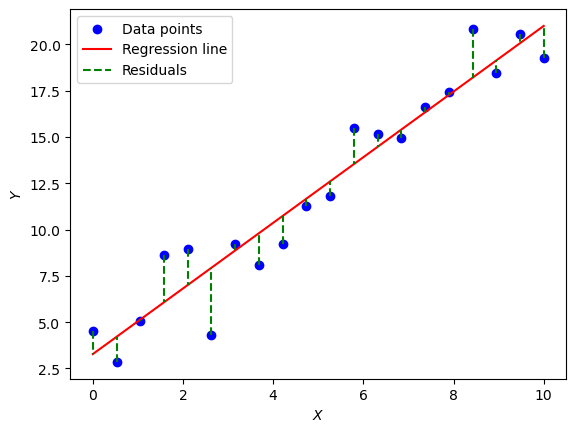
\includegraphics[width=0.8\linewidth]{images/residuals.png}
    \caption{\centering Illustrative example of residuals in the context of linear regression.}
    \label{fig:1.1}
\end{figure}
Using the residuals, we can measure the goodness of fit. We aim to define the linear relation to be as close as possible to the training data. In matrix notation, we can represent the residuals 
for all $n$ available observations as $Y - \textbf{X}\bm{\hat{\beta}}$. To ensure that large errors are penalised more heavily and all of the residuals 
contribute positively, regardless of their sign, the general error function is defined as
\begin{equation}
    \label{equation:1.4}
    (\bm{Y} - \textbf{X}\bm{\hat{\beta}})^T(\bm{Y} - \textbf{X}\bm{\hat{\beta}}).
\end{equation}

Based on Equation \ref{equation:1.4}, we can derive an optimization approach to derive $\hat{\beta}\approx\beta$ as

\begin{equation}
    \label{eq:1.5}
    \min_{\hat{\beta}} \> (\bm{Y} - \textbf{X}\bm{\hat{\beta}})^T(\bm{Y} - \textbf{X}\bm{\hat{\beta}}).
\end{equation}

The approach in Equation \ref{eq:1.5} stands for \textbf{least-squares estimation}. 
Other estimation methods for $\hat{\beta}$ exist; however, only the least-squares approach is included in the chapter, as it is used in the subsequent computational implementation.

\section{Regularized variants of linear regression}

Linear regression commonly tends to overfit certain types of datasets. This problem results in significantly
large values of the parameters in $\bm{\beta}$. Relatively large values of the parameters result in significant changes of predictions
$\hat{Y}$, thus making predictions potentially numerically unstable. There exists a plenty of methods involving explicit feature selection, resulting
in omitting the features with large $\hat{\beta}$; however, this could be avoided \cite{islp}.

Continue with Equation \ref{eq:1.5} and let's add a specific term taking into account the absolute values of the single parameters $\hat{\beta}$  
\begin{equation}
    \label{equation:1.6}
     \min_{\hat{\beta}} \> (\bm{Y} - \textbf{X}\bm{\hat{\beta}})^T(\bm{Y} - \textbf{X}\bm{\hat{\beta}}) + \lambda \|\bm{\hat{\beta}}\|_1,
\end{equation}
where $\lambda \geq 0$ is a so-called tuning parameter. Equation \ref{equation:1.6} trades off two criteria – on the one hand, equally as in linear regression, the model seeks
$\bm{\hat{\beta}}$ which fits the data the best, but on the other hand, the model seeks a fit with the smallest possible absolute values of the elements in $\bm{\hat{\beta}}$.
This method is called \textbf{Lasso regularization} of linear regression and fully aligns with the objectives of preserving all the features, while limiting the possibility of overfitting 
by minimizing the parameters in $\bm{\hat{\beta}}$.

Lasso regularization, while optimizing, might set some of the parameters exactly to zero, which results in a \textbf{feature selection} process and the elimination of potentially invaluable features. 
\newline
\par
Building up on the method introduced by Equation \ref{equation:1.6}, it is possible to use another type of norm to penalize values of the parameters in $\bm{\hat{\beta}}$.
\begin{equation}
    \label{equation:1.7}
     \min_{\hat{\beta}} \> (\bm{Y} - \textbf{X}\bm{\hat{\beta}})^T(\bm{Y} - \textbf{X}\bm{\hat{\beta}}) + \lambda \|\bm{\hat{\beta}}\|_2^2,
\end{equation}
where $\lambda \geq 0$ is again a tuning parameter. In this approach, possibly larger penalty for larger values of $\hat{\beta}$ could be applied, which naturally might result in 
a more strict minimization of their values – minimizing the chance of overfit. The approach in Equation \ref{equation:1.7} is then called \textbf{Ridge regularization} of linear regression.
The aim of this optimization problem aligns with that in Lasso, preserving the trade-off between fit and minimal parameters in $\bm{\hat{\beta}}$. 

Apart from the Lasso, Ridge cannot make the parameters equal to zero, meaning it cannot explicitly perform feature selection.

The most important property of these methods, along with the parameters minimization is the model variance decrease, but an increased bias. This decreases overfit; however, increases the possible error when 
doing approximations on the data. Although, there is an increased possible error, this property makes the model more general and robust \cite{islp,skiena}.

\section{k-Nearest neighbours algorithm}

The main idea, which forms the foundation of this method, is based on the assumption that data points residing in the given vector space, which
are close to each other (for some distance definition), tend to be more similar in terms of the target variable $Y$ \cite{skiena}. This method can solve both regression and classification tasks; however, 
only the regression setup is explained, as only this is used in the thesis.

Suppose we have the training dataset as earlier, $\{ Y_i, \bm{X}_i \}_{i=1}^{n}$, where the stacked vector $\bm{X}_i$ is $(X_{i, 1}, X_{i, 2}, \ldots, X_{i, p})^T$, and $X_{i, q}$ denotes the value of the $q$-th predictor in the $i$-th observation.
Further we have $\bm{\hat{X}}$ composed of the same predictors, but without the linked value of the target $Y$. Lastly, we define a distance metric $\|.\|$ and a parameter $k \leq n$.

Let $N \subseteq \{i\}_{i=1}^{n}$ be the set of indices of the $k$ nearest training feature vectors to the $\bm{\hat{X}}$, in terms of $\|.\|$. Then, the prediction of the target $Y$ is 

\begin{equation}
    Y \approx \frac{1}{k}\sum_{i \in N} Y_i    
\end{equation}

This method is non-parametric and aims to uncover patterns solely using the given training dataset. This method is called the \textbf{k-nearest neighbours} algorithm. 

\section{Random forest algorithm}

\section{Time-series analysis (ARIMA)}